\documentclass[a4paper,12pt]{article}
\usepackage{cmap}
\usepackage[T2A]{fontenc}
\usepackage[utf8]{inputenc}
\usepackage[russian]{babel}
\usepackage{indentfirst}
\usepackage{tikz}
\usetikzlibrary{shapes.misc,shapes.geometric,shapes.multipart,calc,positioning}

\usepackage{geometry}
\geometry{left=3cm}
\geometry{right=2cm}
\geometry{top=2cm}
\geometry{bottom=2cm}

\usepackage[hidelinks]{hyperref}

\usepackage{titletoc}
\newlength{\seclenght}
\settowidth{\seclenght}{6. }
\dottedcontents{section}[\the\seclenght]{}{\the\seclenght}{2mm}
\newlength{\subseclenght}
\settowidth{\subseclenght}{6.2. }
\dottedcontents{subsection}[\the\subseclenght]{}{\the\subseclenght}{2mm}
\newlength{\subsubseclenght}
\settowidth{\subsubseclenght}{6.2.8. }
\dottedcontents{subsubsection}[\the\subsubseclenght]{}{\the\subsubseclenght}{2mm}
\newlength{\pagereflenght}
\settowidth{\pagereflenght}{\pageref{LastPage}}
\contentsmargin{\the\pagereflenght}
\renewcommand{\thesection}{\arabic{section}.}
\renewcommand{\thesubsection}{\thesection\arabic{subsection}.}
\renewcommand{\thesubsubsection}{\thesubsection\arabic{subsubsection}.}
\setcounter{tocdepth}{3}

\usepackage{enumitem}
\usepackage{longtable}
\usepackage{tabu}
\usepackage{lastpage}

\begin{document}
\begin{titlepage}
\begin{center}
\hrule\vspace{1em}
\bf Московский государственный технический университет им. Н.Э.\,Баумана\\
Кафедра <<Системы обработки информации и управления>>\\[1em]
\hrule
\end{center}

\vfill

\noindent УТВЕРЖДАЮ:\\[1em]
\underline{\hspace{12em}} Галкин~В.\,А.\\[1em]
<<\underline{\hspace{1em}}>> \underline{\hspace{6.5em}} 2017~г.

\vfill\vfill

\begin{center}
\large Расчётно-пояснительная записка\\
к~курсовой работе\\
{\Large<<Локальная безадаптерная сеть>>}\\
(вариант №\,26а)\\
по~курсу {\Large<<Сетевые технологии в~АСОИУ>>}
\end{center}

\vfill\vfill\vfill

\begin{tabular*}{\textwidth}{l@{\extracolsep{\fill}}l}
&ИСПОЛНИТЕЛИ:\\[1em]
&\underline{\hspace{12em}} Лещев А.\,О., ИУ5-64\\[1em]
&\underline{\hspace{12em}} Мельников К.\,И., ИУ5-64\\[1em]
&<<\underline{\hspace{1em}}>> \underline{\hspace{6.5em}} 2017~г.\\
\end{tabular*}
 
\vfill

\begin{center}
Москва~--- 2017~г.\\[1em]
\hrule
\end{center}

\end{titlepage}

\setcounter{page}{2}
\tableofcontents
\clearpage

\section{Введение}
Наименование программы: <<Локальная безадаптерная сеть>>. Основанием для~разработки является учебный план кафедры ИУ5 <<Системы обработки информации и управления>> МГТУ им.~Н.Э.\,Баумана на~6~семестр. Исполнителями являются студенты МГТУ им.~Н.Э.\,Баумана группы ИУ5-64 Лещев Артем Олегович и Мельников Константин Игоревич. Программа выполнена на~языке программирования C\# и работает под~управлением операционной системы Microsoft Windows версии 10 или выше.

Программа <<Локальная безадаптерная сеть>>, созданная в~рамках курсовой работы по~курсу <<Сетевые технологии в~АСОИУ>> кафедры ИУ5 <<Системы обработки информации и управления>> МГТУ им.~Н.Э.\,Баумана, позволяет передавать файлы по~локальной сети с~возможностью докачки после восстановления прерванной связи, состоящей из~двух персональных компьютеров, соединённых через интерфейс RS-232C нуль-модемным кабелем.

\subsection{Требования к~программе}
К~программе предъявляются следующие требования:
\begin{enumerate}
\item Программа должна реализовывать разработанные протоколы взаимодействия объектов пользовательского, канального и физического уровней локальной сети.
\item Программа должна защищать передаваемую информацию циклическим кодом $[15,11]$.
\item Программа должна реализовать функцию передачи файлов между двумя персональными компьютерами с~возможностью докачки после восстановления прерванной связи.
\end{enumerate}

\section{Определение структуры программного продукта}
При~взаимодействии компьютеров между собой выделяются несколько уровней: нижний уровень должен обеспечивать передачу, а верхний~--- управление передачей и обеспечение интерфейса пользователя. Программа разбивается на~три уровня: физический, канальный и пользовательский.

Физический уровень предназначен для~сопряжения компьютера со~средой передачи и непосредственной передачи данных по~ней.

Канальный уровень занимается формированием и проверкой кадров, оборачивающих пакеты верхнего уровня.

Пользовательский уровень занимается формированием пакетов и квитанций, обеспечивает изменение интерфейса, выполняет основную задачу программы.

\section{Физический уровень}
\subsection{Функции физического уровня}
Основными функциями физического уровня являются:
\begin{enumerate}
\item установление паpаметpов СОМ-поpта;
\item установление, поддеpжание и pазъединение физического канала;
\item непосредственная передача данных по~каналу.
\end{enumerate}

\subsection{Описание физического уровня}
На~физическом уровне поддерживается передача по~единственной линии с~последовательной передачей данных в~дуплексном канале. При~этом для~синхронизации группе битов данных предшествует специальный стартовый бит, далее после группы битов следует один стоповый бит.

Стартовый бит сигнализирует о начале передачи данных. Далее передаются биты данных. В самом конце передается один стоповый бит, завершающий передачу байта.

Для~корректной передачи данных настройка портов должна быть одинакова как на~стороне приемника, так и на~стороне отправителя. Соответственно, формат данных на~обоих портах должен быть настроен одинаково.

Другая важная характеристика~--- скорость передачи данных. Она также должна быть одинаковой для~передатчика и приемника. Измеряется в~бодах.

Интерфейс RS-232C описывает несимметричный интерфейс, работающий в~режиме последовательного обмена двоичными данными. Интерфейс поддерживает как асинхронный, так и синхронный режимы работы.

Последовательная передача данных означает, что данные передаются по~единственной линии. При~этом биты байта данных передаются по~очереди с~использованием одного провода. Интерфейс называется несимметричным, если для~всех цепей обмена интерфейса используется один общий возвратный провод~--- сигнальная <<земля>>.
Для~определения состояния абонента на~другой стороне кабеля используются другие контакты.

\begin{center}
\begin{tikzpicture}
\node [draw,text width=6ex,align=right] (left) {\texttt{CD\\RxD\\TxD\\DTR\\SG\\DSR\\RTS\\CTS\\RI}};
\node [anchor=north west,text width=6ex] at (left.north west) {\texttt{1\\2\\3\\4\\5\\6\\7\\8\\9}};

\node [draw,text width=6ex,anchor=north west,xshift=15em] (right) at (left.north east) {\texttt{CD\\RxD\\TxD\\DTR\\SG\\DSR\\RTS\\CTS\\RI}};
\node [anchor=north west,text width=6ex,align=right] at (right.north west) {\texttt{1\\2\\3\\4\\5\\6\\7\\8\\9}};

\draw ($(left.north east) + (0em,-0.7em)$) -| node[circle,fill,inner sep=1pt,pos=1] {} ($(left.north east) + (2em,-6.9em)$);
\draw ($(right.north west) + (0em,-0.7em)$) -| node[circle,fill,inner sep=1pt,pos=1] {} ($(right.north west) + (-2em,-6.9em)$);
\draw ($(left.north east) + (0em,-1.9em)$) -- ($(left.north east) + (6em,-1.9em)$) -- ($(left.north east) + (9em,-3.1em)$) -- ($(right.north west) + (0em,-3.1em)$);
\draw ($(left.north east) + (0em,-3.1em)$) -- ($(left.north east) + (6em,-3.1em)$) -- ($(left.north east) + (9em,-1.9em)$) -- ($(right.north west) + (0em,-1.9em)$);
\draw ($(left.north east) + (0em,-4.4em)$) -- ($(left.north east) + (6em,-4.4em)$) -- ($(left.north east) + (9em,-6.9em)$) -- ($(right.north west) + (0em,-6.9em)$);
\draw ($(left.north east) + (0em,-6.9em)$) -- ($(left.north east) + (6em,-6.9em)$) -- ($(left.north east) + (9em,-4.4em)$) -- ($(right.north west) + (0em,-4.4em)$);
\draw ($(left.north east) + (0em,-5.6em)$) -| ($(left.north east) + (6em,-5em)$) -| ($(left.north east) + (9em,-5.6em)$) -- ($(right.north west) + (0em,-5.6em)$);
\draw ($(left.north east) + (0em,-8.1em)$) -- ($(left.north east) + (6em,-8.1em)$) -- ($(left.north east) + (9em,-9.3em)$) -- ($(right.north west) + (0em,-9.3em)$);
\draw ($(left.north east) + (0em,-9.3em)$) -- ($(left.north east) + (6em,-9.3em)$) -- ($(left.north east) + (9em,-8.1em)$) -- ($(right.north west) + (0em,-8.1em)$);
\draw ($(left.north east) + (0em,-10.5em)$) -- ($(left.north east) + (2em,-10.5em)$);
\node [draw,anchor=west] at ($(left.north east) + (2em,-10.5em)$) {$\times$};
\draw ($(right.north west) + (0em,-10.5em)$) -- ($(right.north west) + (-2em,-10.5em)$);
\node [draw,anchor=east] at ($(right.north west) + (-2em,-10.5em)$) {$\times$};
\end{tikzpicture}
\end{center}

Контакт DTR (Data Terminal Ready)~--- готовность к~приёму данных. Означает готовность к~приему данных (физическое соединение).

Контакт RTS (Request to~Send)~--- запрос на передачу. Означает готовность к~приёму данных.

Контакт DSR (Data Set Ready)~--- готовность к~передаче данных.

Контакт CTS (Clear to Send)~--- готовность передачи.

Контакт DCD (Carrier Detect)~--- наличие несущей.

\subsection{Защита передаваемой информации}
Физический уровень получает массив бит, которые следует передать. Для~осуществления надёжной передачи на~данном уровне, массив делится на~группы 11~бит или меньше, которые защищаются циклическим кодом $[15,11]$.

Отобранные 11~бит подвергаются сдвигу влево на~4 бита с~заполнением нулями. Далее полученный массив бит подвергается циклическому делению с~помощью сложения по~модулю~2 с~образующим полиномом $x^4+x+1$, полученный остаток записывается в~4~последних бита.

Обратная операция аналогична. Если остаток (синдром ошибки) от~циклического деления с~помощью сложения по~модулю~2 с~образующим полиномом больше~0, то считается, что обнаружена ошибка. Защита циклическим кодом может исправить 1~бит. Если ошибка больше одного бита, это будет видно по~контрольной сумме на~канальном уровне.

\section{Настройка COM-порта средствами C\#}
Пространство имен \texttt{System.IO.Ports} стандартной библиотеки платформы .NET Framework языка программирования C\# предлагает широкие возможности по~настройке COM-порта.

\subsection{Описание класса \texttt{SerialPort}}
Данный класс используется для~управления файловым ресурсом последовательного порта. Данный класс предоставляет возможности управления вводом-выводом в~синхронном режиме или на~основе событий, доступа к~состоянию линии и состоянию разрыва, а также доступа к~свойствам последовательного драйвера.

\subsubsection*{Методы класса}
\begin{center}
\begin{longtabu} to \linewidth {|X|X[2.6]|}
\hline
\textbf{Имя}	&	\textbf{Описание}\\\hline\endhead
\texttt{Close}	&	Закрывает соединение порта, присваивает свойству \texttt{IsOpen} значение \texttt{false} и уничтожает внутренний объект \texttt{Stream}.\\\hline
\texttt{GetPortNames}	&	Получает массив имен последовательных портов для~текущего компьютера.\\\hline
\texttt{Open}	&	Открывает новое соединение последовательного порта.\\\hline
\texttt{Read(System.Byte[], System.Int32, System.Int32)}	&	Считывает из~входного буфера \texttt{SerialPort} определенное число байтов и записывает их в~байтовый массив, начиная с~указанной позиции.\\\hline
\texttt{ReadByte}	&	Считывает из~входного буфера \texttt{SerialPort} один байт в~синхронном режиме.\\\hline
\texttt{DiscardInBuffer}	&	Удаляет данные из~буфера приема последовательного драйвера\\\hline
\texttt{DiscardOutBuffer}	&	Удаляет данные из~буфера передачи последовательного драйвера\\\hline
\texttt{Write(System.String)}	&	Записывает указанную строку в~последовательный порт.\\\hline
\end{longtabu}
\end{center}

\subsubsection*{Свойства класса}
\begin{center}
\begin{longtabu} to \linewidth {|X|X[2.7]|}
\hline
\textbf{Имя}	&	\textbf{Описание}\\\hline\endhead
\texttt{BaudRate}	&	Получает или задает скорость передачи для последовательного порта (в~бодах).\\\hline
\texttt{BreakState}	&	Получает или задает состояние сигнала разрыва.\\\hline
\texttt{BytesToRead}	&	Получает число байтов данных, находящихся в~буфере приема.\\\hline
\texttt{BytesToWrite}	&	Получает число байтов данных, находящихся в~буфере отправки.\\\hline
\texttt{CDHolding}	&	Получает состояние линии обнаружения несущей для~порта.\\\hline
\texttt{CtsHolding}	&	Получает состояние линии готовности к~приему.\\\hline
\texttt{DataBits}	&	Получает или задает стандартное число битов данных в~байте.\\\hline
\texttt{DsrHolding}	&	Получает или задает состояние сигнала готовности данных (DSR).\\\hline
\texttt{DtrEnable}	&	Получает или задает значение, включающее поддержку сигнала готовности терминала (DTR) в~сеансе последовательной связи.\\\hline
\texttt{Encoding}	&	Получает или задает кодировку байтов для~преобразования текста до и после передачи.\\\hline
\texttt{Events}	&	Возвращает список обработчиков событий, которые прикреплены к~этому объекту \texttt{Component} (унаследовано от~\texttt{Component}).\\\hline
\texttt{IsOpen}	&	Получает значение, указывающее состояние объекта \texttt{SerialPort}~--- открыт или закрыт.\\\hline
\texttt{Parity}	&	Получает или задает протокол контроля четности.\\\hline
\texttt{PortName}	&	Получает или задает последовательный порт, в~частности, любой из~доступных портов COM.\\\hline
\texttt{ReadBufferSize}	&	Получает или задает размер входного буфера \texttt{SerialPort}.\\\hline
\texttt{RtsEnable}	&	Получает или задает значение, показывающее, включен ли сигнал запроса передачи (RTS) в~сеансе последовательной связи.\\\hline
\texttt{StopBits}	&	Получает или задает стандартное число стоповых битов в~байте.\\\hline
\texttt{WriteBufferSize}	&	Получает или задает размер выходного буфера последовательного порта. \\\hline
\end{longtabu}
\end{center}

\subsubsection*{События класса}
\begin{center}
\begin{longtabu} to \linewidth {|X|X[2.6]|}
\hline
\textbf{Имя}	&	\textbf{Описание}\\\hline\endhead
\texttt{DataReceived}	&	Представляет метод обработки события получения данных для~объекта \texttt{SerialPort}.\\\hline
\texttt{ErrorReceived}	&	Представляет метод обработки ошибок объекта \texttt{SerialPort}.\\\hline
\texttt{PinChanged}	&	Представляет метод обработки события изменения состояния контактов для~объекта \texttt{SerialPort}.\\\hline
\end{longtabu}
\end{center}

\subsection{Описание класса \texttt{Physical}}
Данный класс был разработан в~ходе работы над~данной программы для~реализации её физического уровня.

\subsubsection*{Поля класса}
\begin{center}
\begin{longtabu} to \linewidth {|X|X[2.6]|}
\hline
\textbf{Имя}	&	\textbf{Описание}\\\hline\endhead
\texttt{\_serialPort}	&	Экземпляр объекта \texttt{SerialPort}.\\\hline
\texttt{connected}	&	Состояние подключения.\\\hline
\texttt{failList}	&	Список синдромов ошибок циклического кода $[15,11]$.\\\hline
\end{longtabu}
\end{center}

\subsubsection*{События класса}
\begin{center}
\begin{longtabu} to \linewidth {|X|X[2.6]|}
\hline
\textbf{Имя}	&	\textbf{Описание}\\\hline\endhead
\texttt{OnCheck}	&	Событие, срабатывающее при~изменении состояния COM-порта.\\\hline
\texttt{UICheck}	&	Событие, отправляющее состояние порта при~попытке отправки группы байт.\\\hline
\end{longtabu}
\end{center}

\subsubsection*{Методы класса}
\begin{center}
\begin{longtabu} to \linewidth {|X|X[2.6]|}
\hline
\textbf{Имя}	&	\textbf{Описание}\\\hline\endhead
\texttt{SetRts}	&	Позволяет выставлять контакт RTS.\\\hline
\texttt{StatusCheck}	&	Обработчик изменения состояния COM-порта.\\\hline
\texttt{Connect}	&	Метод подключения к~COM-порту.\\\hline
\texttt{Disconnect}	&	Метод отключения от~COM-порта.\\\hline
\texttt{DataReceivedHandler}	&	Обработчик события получения байт.\\\hline
\texttt{DeCycle}	&	Метод для~декодирования циклического кода $[15,11]$.\\\hline
\texttt{Send}	&	Метод для~отправки кадра.\\\hline
\texttt{GetCycled}	&	Метод, кодирующий данные циклическим кодом $[15,11]$.\\\hline
\end{longtabu}
\end{center}

\section{Канальный уровень}
\subsection{Функции канального уровня}
На~канальном уровне выполняются следующие функции:
\begin{enumerate}
\item упpавление пеpедачей кадpов;
\item обеспечение необходимой последовательности блоков данных, пеpедаваемых чеpез межуpовневый интеpфейс;
\item контpоль и исправление ошибок.
\end{enumerate}

Канальный уровень управляет передачей кадров, но не~гарантирует их доставку. Управление соединением осуществляется через пакеты на~пользовательском уровне.

Канальный уровень получает массив байт (пакет), экранирует все байты \texttt{0xFE} и \texttt{0xFE}, считает проверочную сумму, добавляет её в~начало кадра. Добавляет стартовый и стоповый байты кадра. После этого кадр отправляется на~физический уровень.

\subsection{Описание класса \texttt{DataLink}}
Данный класс был разработан в~ходе работы над~данной программы для~реализации её канального уровня.

\subsubsection*{Поля класса}
\begin{center}
\begin{longtabu} to \linewidth {|X|X[2.6]|}
\hline
\textbf{Имя}	&	\textbf{Описание}\\\hline\endhead
\texttt{currentPacket}	&	Пакет для~отправки.\\\hline
\texttt{checkSumm}	&	Проверочная сумма, посчитанная на~основе пакета.\\\hline
\texttt{length}	&	Длина пакета.\\\hline
\texttt{firstTrigger}	&	Триггер, показывающий, работает ли в~данный момент канальный уровень с~пакетом.\\\hline
\texttt{secondTrigger}	&	Триггер, показывающий, получен ли пакет полностью.\\\hline
\texttt{screenTrigger}	&	Триггер, показывающий, был ли предыдущий байт экранирован.\\\hline
\texttt{recievedPacket}	&	Список байтов, полученных от~физического уровня.\\\hline
\texttt{recievedPacketBuffer}	&	Промежуточный список битов, полученных от~физического уровня.\\\hline
\texttt{debugBuffer}	&	Отладочный буфер битов, полученных от~физического уровня.\\\hline
\end{longtabu}
\end{center}

\subsubsection*{Методы класса}
\begin{center}
\begin{longtabu} to \linewidth {|X|X[2.6]|}
\hline
\textbf{Имя}	&	\textbf{Описание}\\\hline\endhead
\texttt{DataLink}	&	Конструктор класса.\\\hline
\texttt{TimerListener}	&	Функция, определяющая, необходимо ли очистить буфер по~истечении таймера.\\\hline
\texttt{RecievePacket}	&	Функция, вызываемая физическим уровнем для~обработки полученных бит.\\\hline
\texttt{SendPacket}	&	Функция, формирующая из~пакета кадр и отправляющая его на~физический уровень.\\\hline
\end{longtabu}
\end{center}

\subsection{Формат кадра}
\begin{center}
\begin{tikzpicture}[every node/.style={draw,align=center}]
\node [rectangle split,rectangle split horizontal,rectangle split parts=4] (Frame) {\parbox{7em}{\centering\texttt{11111111}}\nodepart{two}\parbox{10em}{\centering$\sum_{i=1}^m\mathtt{newPacket}[i]$}\nodepart{three}\texttt{newPacket}\nodepart{four}\parbox{7em}{\centering\texttt{11111111}}};
\node [anchor=south,draw=none] (FrameField1) at (Frame.one north) {Стартовый байт};
\node [anchor=south,draw=none] (FrameField2) at (Frame.two north) {Контрольная сумма};
\node [anchor=south,draw=none] (FrameField3) at (Frame.three north) {Пакет};
\node [anchor=south,draw=none] (FrameField4) at (Frame.four north) {Стоповый байт};
\draw (Frame.north west) -- ($(Frame.south west) + (0,-2em)$);
\draw (Frame.one split south) -- ($(Frame.one split south) + (0,-2em)$);
\draw [latex-latex] ($(Frame.south west) + (0,-1.5em)$) -- node [above,draw=none] {1 байт} ($(Frame.one split south) + (0,-1.5em)$);
\draw (Frame.two split south) -- ($(Frame.two split south) + (0,-2em)$);
\draw [latex-latex] ($(Frame.one split south) + (0,-1.5em)$) -- node [above,draw=none] {4 байта} ($(Frame.two split south) + (0,-1.5em)$);
\draw (Frame.three split south) -- ($(Frame.three split south) + (0,-2em)$);
\draw [latex-latex] ($(Frame.two split south) + (0,-1.5em)$) -- node [above,draw=none] {$m$ байтов} ($(Frame.three split south) + (0,-1.5em)$);
\draw (Frame.north east) -- ($(Frame.south east) + (0,-2em)$);
\draw [latex-latex] ($(Frame.three split south) + (0,-1.5em)$) -- node [above,draw=none] {1 байт} ($(Frame.south east) + (0,-1.5em)$);
\end{tikzpicture}
\end{center}

\section{Пользовательский уровень}
Функции пользовательского уровня обеспечивает интерфейс программы через форму. Пользовательский уровень предоставляет нижнему уровню пакет для~отправки.

На данном уровне обеспечивается выбор файла и папки, отображение статуса COM-порта и передачи файла, вывод системных сообщений.

\subsection{Описание интерфейса}
Пользовательский интерфейс выполнен в~среде Microsoft Visual Studio с~использованием библиотеки Windows Presentation Foundation.

Основным окном программы является окно «Локальная безадаптерная сеть». В данной форме есть следующие возможности:
\begin{itemize}
\item выбор COM-порта;
\item открытие COM-порта;
\item закрытие COM-порта;
\item мониторинг состояния контактов COM-порта;
\item выбор файла для~отправки;
\item отправка файла;
\item выбор папки для~приёма файла;
\item мониторинг состояния передачи файла;
\item разъединение логического соединения.
\end{itemize}
\begin{center}
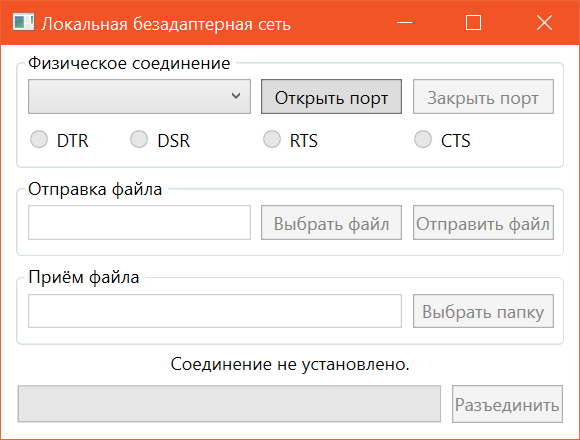
\includegraphics{window.png};
\end{center}

При~открытии списка отображается список доступных COM-портов.
\begin{center}
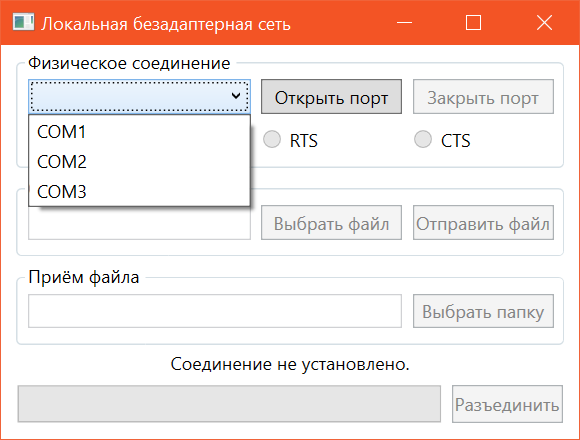
\includegraphics{list.png};
\end{center}
При~нажатии на~кнопку <<Открыть порт>> происходит открытие порта. При~нажатии кнопки «Закрыть порт» происходит закрытие порта.

При~нажатии на~кнопку <<Выбрать файл>>, открывается стандартное окно выбора файла.
\begin{center}
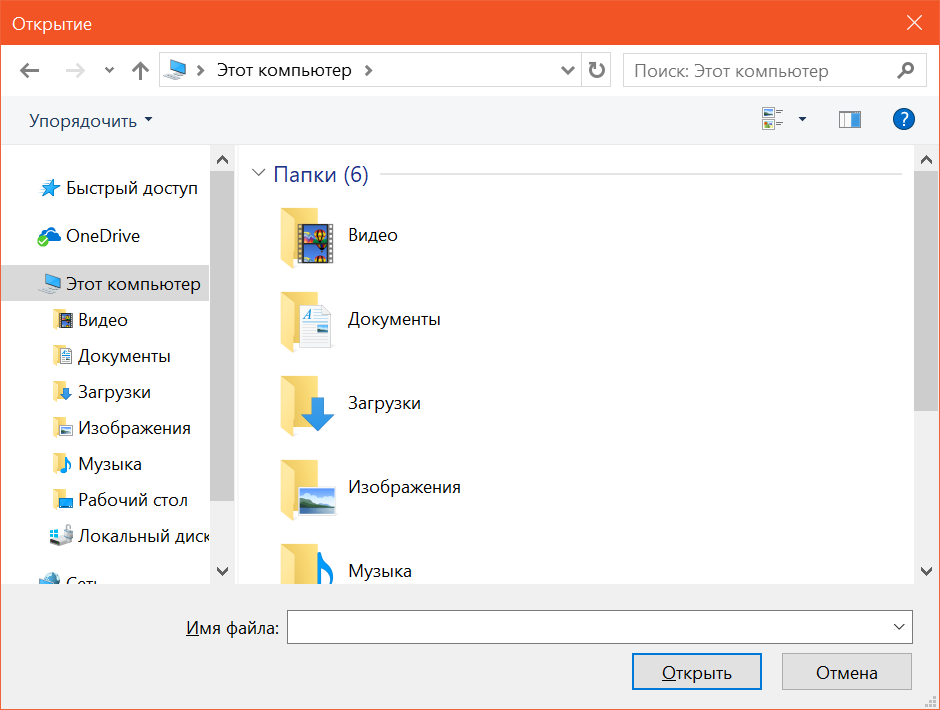
\includegraphics[width=\linewidth]{file.png};
\end{center}

При~нажатии на~кнопку <<Выбрать папку>>, открывается стандартное окно выбора папки.
\begin{center}
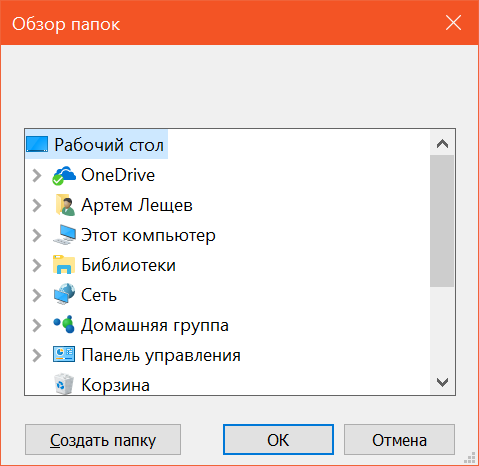
\includegraphics{folder.png};
\end{center}

После нажатия на~кнопку <<Отправить файл>> происходит отправка файла. Процесс отправки отображается индикатором.
\begin{center}
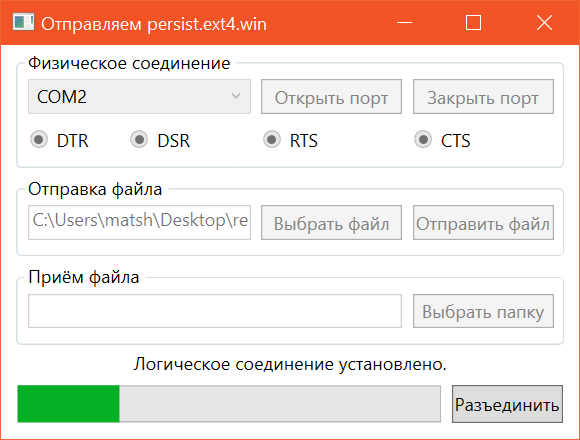
\includegraphics{progress.png};
\end{center}

Нажатием кнопки <<Разъединить>> можно досрочно прервать передачу файла. После этого можно возобновить передачу, снова нажав кнопку <<Отправить файл>>.

\subsection{Форматы пакетов}
\begin{enumerate}
\item Пакет данных о~файле

\begin{tikzpicture}[every node/.style={draw,align=center}]
\node [rectangle split,rectangle split horizontal,rectangle split parts=4] (FileName) {\texttt{00000000}\nodepart{two}\texttt{fileDialog.SafeFileName}\nodepart{three}\texttt{fileStream.Length}\nodepart{four}$\mathrm{SHA512}(\mathtt{fileStream})$};
\node [anchor=south,draw=none] (FileNameField1) at (FileName.one north) {Тип пакета};
\node [anchor=south,draw=none] (FileNameField2) at (FileName.two north) {Имя файла};
\node [anchor=south,draw=none] (FileNameField3) at (FileName.three north) {Длина файла};
\node [anchor=south,draw=none] (FileNameField4) at (FileName.four north) {Контрольная сумма};
\draw (FileName.north west) -- ($(FileName.south west) + (0,-2.5em)$);
\draw (FileName.one split south) -- ($(FileName.one split south) + (0,-2.5em)$);
\draw [latex-latex] ($(FileName.south west) + (0,-2em)$) -- node [above,draw=none] {1 байт} ($(FileName.one split south) + (0,-2em)$);
\draw (FileName.two split south) -- ($(FileName.two split south) + (0,-2.5em)$);
\draw [latex-latex] ($(FileName.one split south) + (0,-2em)$) -- node [above,draw=none] {$(k + \lfloor\log_{128}k\rfloor + 1)$ байтов} ($(FileName.two split south) + (0,-2em)$);
\draw (FileName.three split south) -- ($(FileName.three split south) + (0,-2.5em)$);
\draw [latex-latex] ($(FileName.two split south) + (0,-2em)$) -- node [above,draw=none] {8 байтов} ($(FileName.three split south) + (0,-2em)$);
\draw (FileName.north east) -- ($(FileName.south east) + (0,-2.5em)$);
\draw [latex-latex] ($(FileName.three split south) + (0,-2em)$) -- node [above,draw=none] {64 байта} ($(FileName.south east) + (0,-2em)$);
\end{tikzpicture}

\clearpage
\item Пакет неготовности к~получению файла

\begin{tikzpicture}[every node/.style={draw,align=center}]
\node (ReceiveNotReady) {\texttt{00000001}};
\node [anchor=south,draw=none] (ReceiveNotReadyField1) at (ReceiveNotReady.north) {Тип пакета};
\draw (ReceiveNotReady.north west) -- ($(ReceiveNotReady.south west) + (0,-2.5em)$);
\draw (ReceiveNotReady.north east) -- ($(ReceiveNotReady.south east) + (0,-2.5em)$);
\draw [latex-latex] ($(ReceiveNotReady.south west) + (0,-2em)$) -- node [above,draw=none] {1 байт} ($(ReceiveNotReady.south east) + (0,-2em)$);
\end{tikzpicture}

\item Пакет запроса части файла

\begin{tikzpicture}[every node/.style={draw,align=center}]
\node [rectangle split,rectangle split horizontal,rectangle split parts=2] (FileRequest) {\texttt{00000002}\nodepart{two}\texttt{fileStream.Length}};
\node [anchor=south,draw=none] (FileRequestField1) at (FileRequest.one north) {Тип пакета};
\node [anchor=south,draw=none] (FileRequestField2) at (FileRequest.two north) {Позиция};
\draw (FileRequest.north west) -- ($(FileRequest.south west) + (0,-2.5em)$);
\draw (FileRequest.one split south) -- ($(FileRequest.one split south) + (0,-2.5em)$);
\draw [latex-latex] ($(FileRequest.south west) + (0,-2em)$) -- node [above,draw=none] {1 байт} ($(FileRequest.one split south) + (0,-2em)$);
\draw (FileRequest.north east) -- ($(FileRequest.south east) + (0,-2.5em)$);
\draw [latex-latex] ($(FileRequest.one split south) + (0,-2em)$) -- node [above,draw=none] {8 байтов} ($(FileRequest.south east) + (0,-2em)$);
\end{tikzpicture}

\item Пакет части файла

\begin{tikzpicture}[every node/.style={draw,align=center}]
\node [rectangle split,rectangle split horizontal,rectangle split parts=4] (FileChunk) {\texttt{00000003}\nodepart{two}Позиция в~файле\nodepart{three}\parbox{5em}{\centering$n$}\nodepart{four}\parbox{7em}{\centering Данные}};
\node [anchor=south,draw=none] (FileChunkField1) at (FileChunk.one north) {Тип пакета};
\node [anchor=south,draw=none] (FileChunkField2) at (FileChunk.two north) {Позиция};
\node [anchor=south,draw=none] (FileChunkField3) at (FileChunk.three north) {Размер части};
\node [anchor=south,draw=none] (FileChunkField4) at (FileChunk.four north) {Часть файла};
\draw (FileChunk.north west) -- ($(FileChunk.south west) + (0,-2.5em)$);
\draw (FileChunk.one split south) -- ($(FileChunk.one split south) + (0,-2.5em)$);
\draw [latex-latex] ($(FileChunk.south west) + (0,-2em)$) -- node [above,draw=none] {1 байт} ($(FileChunk.one split south) + (0,-2em)$);
\draw (FileChunk.two split south) -- ($(FileChunk.two split south) + (0,-2.5em)$);
\draw [latex-latex] ($(FileChunk.one split south) + (0,-2em)$) -- node [above,draw=none] {8 байтов} ($(FileChunk.two split south) + (0,-2em)$);
\draw (FileChunk.three split south) -- ($(FileChunk.three split south) + (0,-2.5em)$);
\draw [latex-latex] ($(FileChunk.two split south) + (0,-2em)$) -- node [above,draw=none] {2 байта} ($(FileChunk.three split south) + (0,-2em)$);
\draw (FileChunk.north east) -- ($(FileChunk.south east) + (0,-2.5em)$);
\draw [latex-latex] ($(FileChunk.three split south) + (0,-2em)$) -- node [above,draw=none] {$n$ байтов} ($(FileChunk.south east) + (0,-2em)$);
\end{tikzpicture}

\item Пакет квитанции о~получении файла

\begin{tikzpicture}[every node/.style={draw,align=center}]
\node (FileReceived) {\texttt{00000004}};
\node [anchor=south,draw=none] (FileReceivedField1) at (FileReceived.north) {Тип пакета};
\draw (FileReceived.north west) -- ($(FileReceived.south west) + (0,-2.5em)$);
\draw (FileReceived.north east) -- ($(FileReceived.south east) + (0,-2.5em)$);
\draw [latex-latex] ($(FileReceived.south west) + (0,-2em)$) -- node [above,draw=none] {1 байт} ($(FileReceived.south east) + (0,-2em)$);
\end{tikzpicture}

\item Пакет квитанции о~завершении передачи

\begin{tikzpicture}[every node/.style={draw,align=center}]
\node (FileReceivedOk) {\texttt{00000005}};
\node [anchor=south,draw=none] (FileReceivedOkField1) at (FileReceivedOk.north) {Тип пакета};
\draw (FileReceivedOk.north west) -- ($(FileReceivedOk.south west) + (0,-2.5em)$);
\draw (FileReceivedOk.north east) -- ($(FileReceivedOk.south east) + (0,-2.5em)$);
\draw [latex-latex] ($(FileReceivedOk.south west) + (0,-2em)$) -- node [above,draw=none] {1 байт} ($(FileReceivedOk.south east) + (0,-2em)$);
\end{tikzpicture}

\item Пакет разрыва соединения

\begin{tikzpicture}[every node/.style={draw,align=center}]
\node (Disconnect) {\texttt{00000006}};
\node [anchor=south,draw=none] (DisconnectField1) at (Disconnect.north) {Тип пакета};
\draw (Disconnect.north west) -- ($(Disconnect.south west) + (0,-2.5em)$);
\draw (Disconnect.north east) -- ($(Disconnect.south east) + (0,-2.5em)$);
\draw [latex-latex] ($(Disconnect.south west) + (0,-2em)$) -- node [above,draw=none] {1 байт} ($(Disconnect.south east) + (0,-2em)$);
\end{tikzpicture}

\item Пакет квитанции о~разрыве соединения

\begin{tikzpicture}[every node/.style={draw,align=center}]
\node (DisconnectOk) {\texttt{00000007}};
\node [anchor=south,draw=none] (DisconnectOkField1) at (DisconnectOk.north) {Тип пакета};
\draw (DisconnectOk.north west) -- ($(DisconnectOk.south west) + (0,-2.5em)$);
\draw (DisconnectOk.north east) -- ($(DisconnectOk.south east) + (0,-2.5em)$);
\draw [latex-latex] ($(DisconnectOk.south west) + (0,-2em)$) -- node [above,draw=none] {1 байт} ($(DisconnectOk.south east) + (0,-2em)$);
\end{tikzpicture}
\end{enumerate}

\end{document}